% vi:ft=tex
\documentclass[utf8,10pt]{beamer}

\usepackage[english]{babel}
\usepackage{etex}
\usepackage{pgf}
\usepackage[absolute,overlay]{textpos}
\usepackage{tikz}
\usepackage{listings}
\usepackage{graphicx}
\usepackage{pgfplots}
\usepackage{standalone}
\usepackage{enumitem}
%\usepackage[bitstream-charter]{mathdesign}
\usepackage{berasans}
\usepackage[backend=biber,style=alphabetic]{biblatex}
\usepackage{multirow}
\usepackage{mathtools}
\usepackage{ragged2e}
\usepackage{minted}
\usepackage{verbatim}
\usepackage{amssymb}
\usepackage{amsfonts}
\usepackage{textcomp}

\usetikzlibrary{arrows, shapes, positioning, trees,calc,intersections}
\mode<presentation>

% 45 degree rotated column descriptor
\usepackage{adjustbox}
\usepackage{array}

\usetheme[noheader,smallrightmargin,smallleftmargin,nosectionnum,heavyfont,pagenum]{tud}
\addbibresource{./Related_Work.bib}

\setbeamertemplate{footnote}
{
  %\scriptsize
  \tiny
  \noindent%
  \insertfootnotemark~\insertfootnotetext
}

\setbeamertemplate{enumerate items}[default]
\setbeamertemplate{itemize items}[triangle]

\title[]{Multicore Load Balancing based on behaviour observation on \textmu--kernels}

\author{Philipp Eppelt}

\date{20.11.2015}
\datecity{Dresden}

\einrichtung{Fakult\"a{}t Informatik}

\institut{Institut f\"u{}r Systemarchitektur}
\professur{Lehrstuhl f\"u{}r Betriebssysteme}


\begin{document}

\maketitle

\large

\newcommand{\ft}[1]{\frametitle{\hfill #1}}

% motivation
%%%%%%%%%%%%%%%%%%%%%%%%%%%%%%%%%%%%%%%%%%%%%%%%%%%%%%%%%%%%%%%%%%%%%%%%%%%%%%

\begin{frame}
  \frametitle{fiasco does no balancing \& \\ run-queue balancing disregards
  item size}
  \centering
  \begin{minipage}[l]{.49\columnwidth}
    \includestandalone[width=\columnwidth]{./scheduling_curr_fiasco}
  \end{minipage}
  \begin{minipage}[r]{.49\columnwidth}
    \includestandalone[width=\columnwidth]{./scheduling_curr_rq}
  \end{minipage}
\end{frame}


\begin{frame}
  \frametitle{observe thread's time \& cache usage \\ and balance these}
  \centering
  \begin{minipage}[l]{.49\columnwidth}
    \includestandalone[width=\columnwidth]{./scheduling_curr_bal_time}
  \end{minipage}
  \begin{minipage}[r]{.49\columnwidth}
    \includestandalone[width=\columnwidth]{./scheduling_curr_bal_cache}
  \end{minipage}
\end{frame}


% state of the art
%%%%%%%%%%%%%%%%%%%%%%%%%%%%%%%%%%%%%%%%%%%%%%%%%%%%%%%%%%%%%%%%%%%%%%%%%%%%%%
% SMT

\begin{frame}
  \frametitle{three concepts to approach distribution}
  \begin{itemize}
    \item offline measurement --- online distribution
      \footfullcite{eyerman_revisiting_2015}
    \item online measurement --- online symbiosis
      \footfullcite{snavely_symbiotic_2000} \footfullcite{banikazemi_pam_2008}
    \item intertwined online measurement and adaption
      \footfullcite{knauerhase_using_2008} \footfullcite{zhuravlev_addressing_2010}
  \end{itemize}
\end{frame}


\begin{frame}
  \frametitle{performance metrics \\should not depend on system load
    \footfullcite{eyerman_revisiting_2015}}
  \centering
  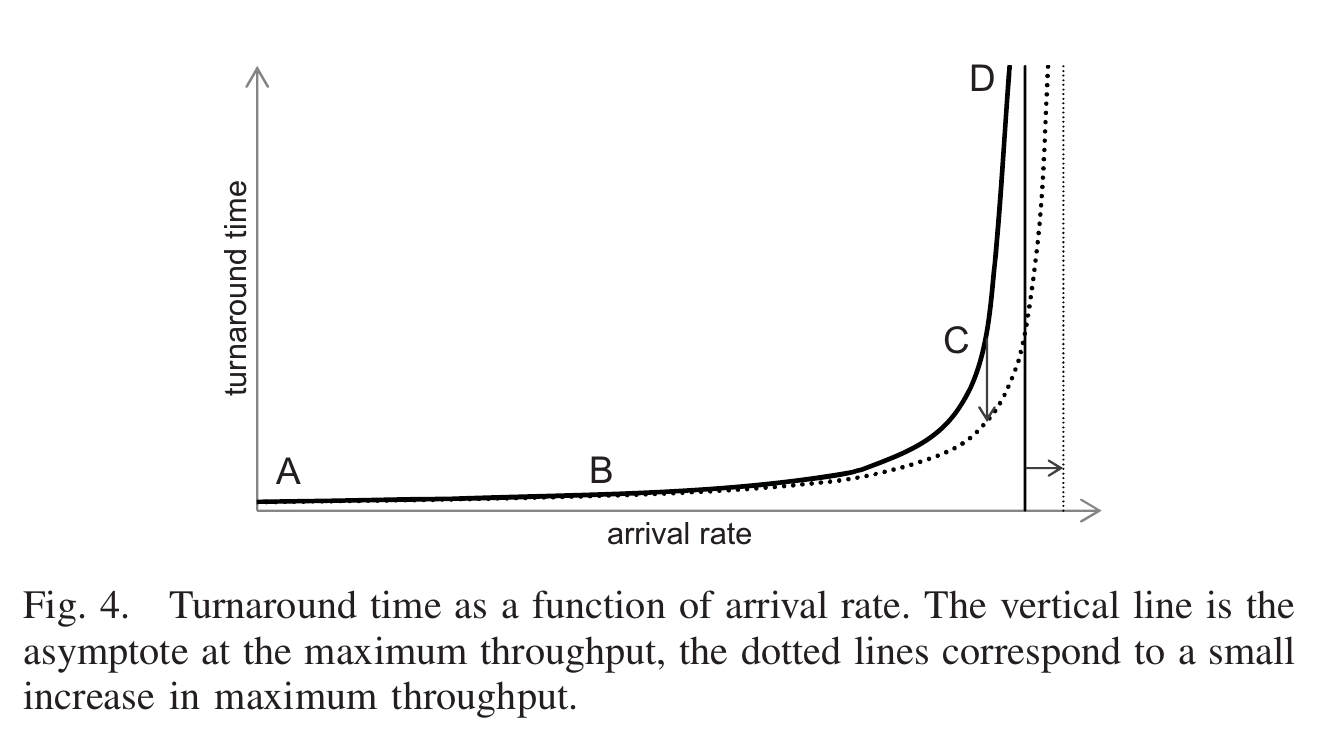
\includegraphics[height=0.7\textheight, keepaspectratio]{./arrival_rate}
\end{frame}


\begin{frame}
  \frametitle{performance metrics\footfullcite{eyerman_revisiting_2015}}
  \begin{minipage}[l]{.49\columnwidth}
    \centering
    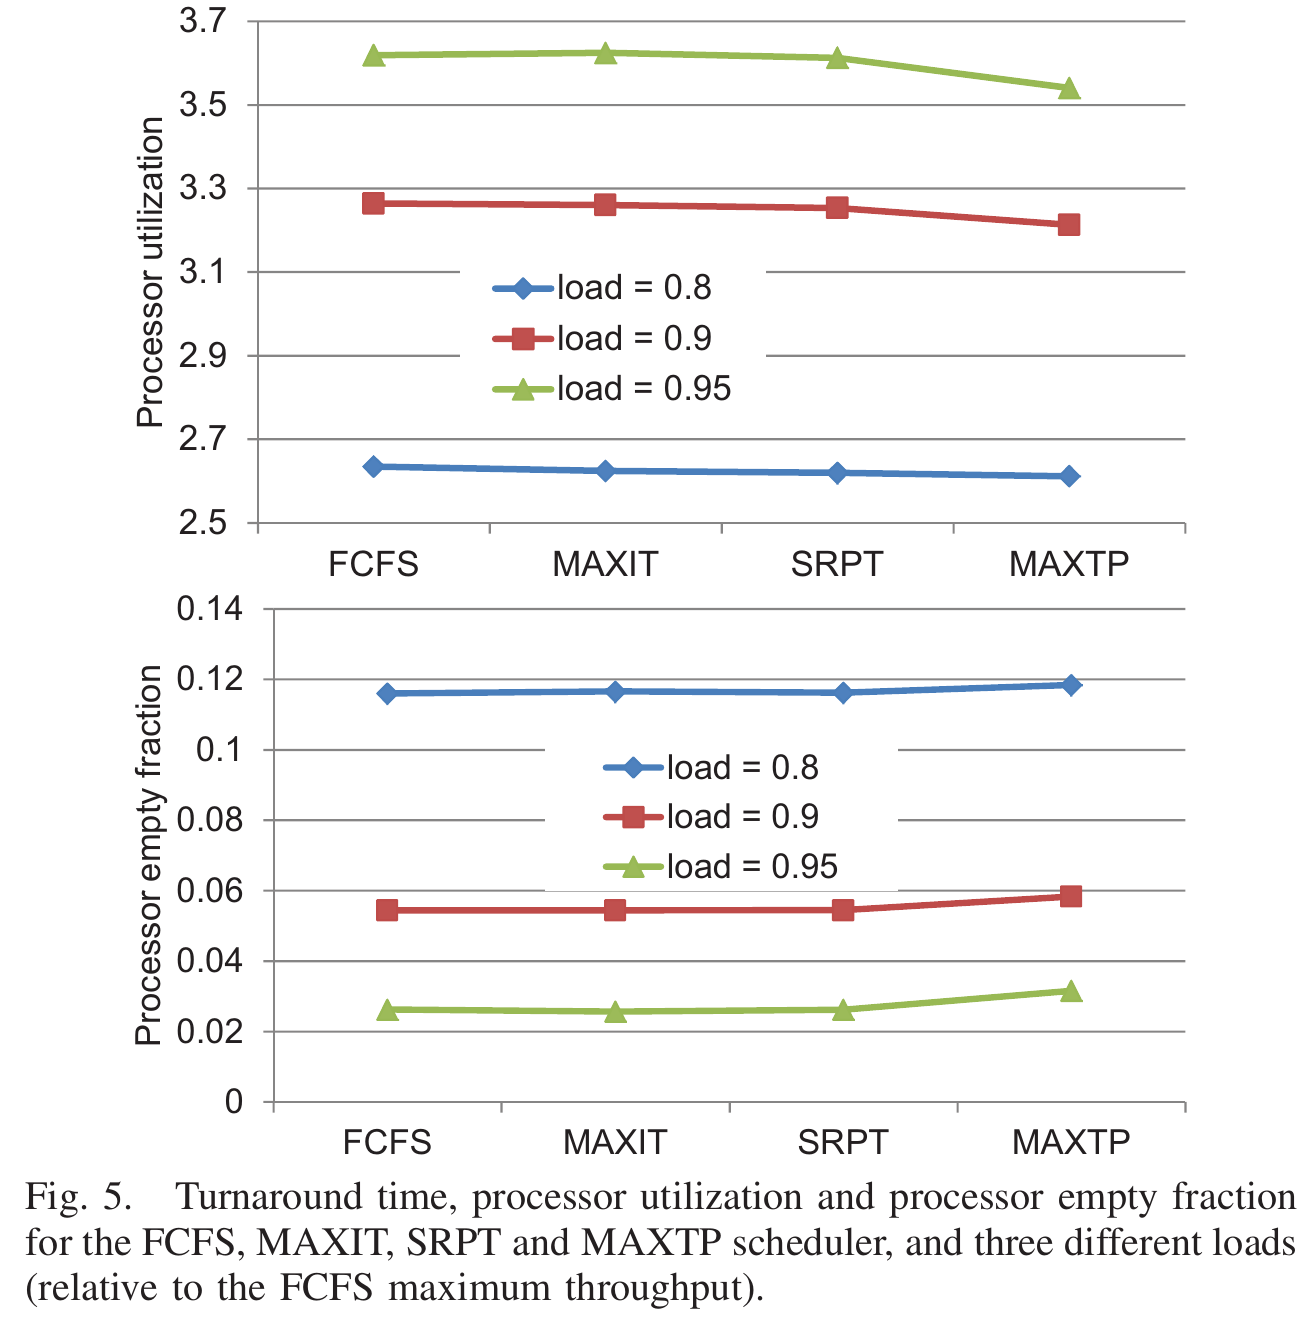
\includegraphics[height=0.7\textheight,
    keepaspectratio]{./empty_utilization_comparison_bottom}
  \end{minipage}
  \begin{minipage}[r]{.49\columnwidth}
    \centering
    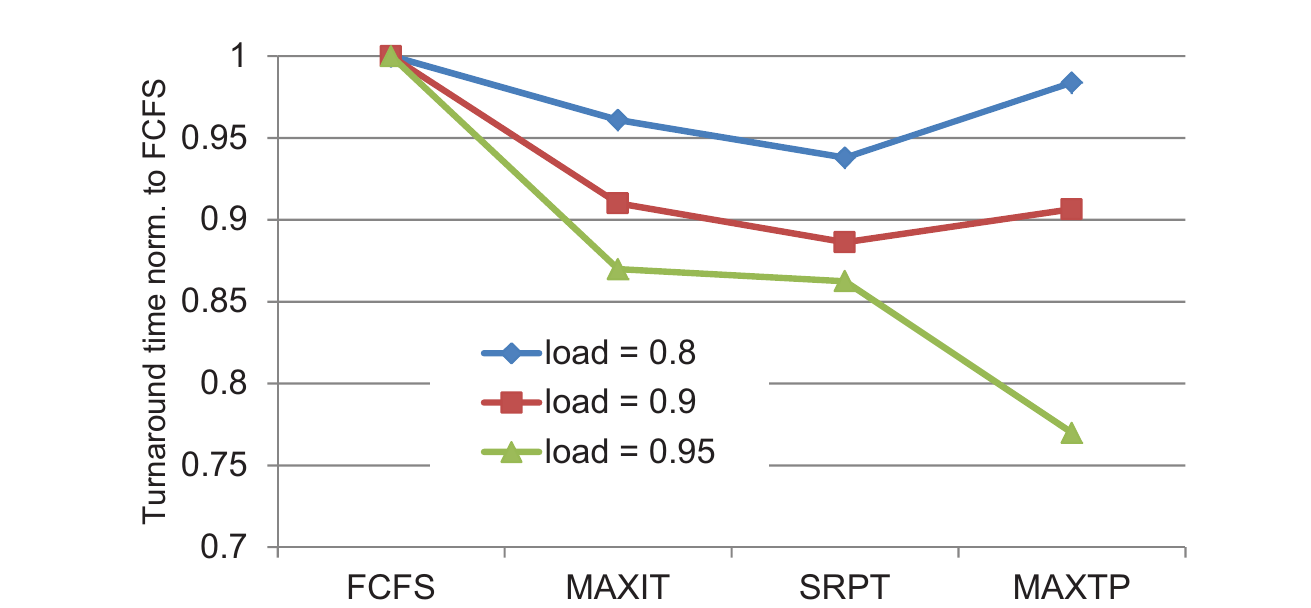
\includegraphics[width=\columnwidth,
    keepaspectratio]{./empty_utilization_comparison_top}
  \end{minipage}
\end{frame}


% cache observation
\begin{frame}
  \frametitle{contention sources \footfullcite{fedorova_managing_2010}}
  \centering
  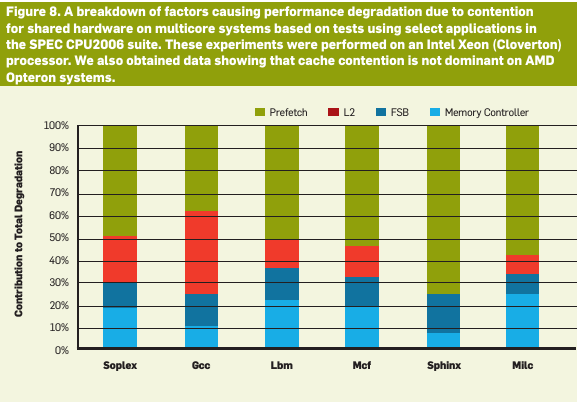
\includegraphics[height=0.7\textheight, keepaspectratio]{./contention_shared_hw}
\end{frame}


\begin{frame}
  \frametitle{pain metric combines sensitivity to cache
    changes with the intensity of cache usage\footfullcite{zhuravlev_addressing_2010}}
  \centering
  \begin{align*}
    Pain(A|B) &= sensitivity(A) * intensity(B) \\
    Pain(B|A) &= sensitivity(B) * intensity(A) \\
    Pain(A,B) &= Pain(A|B) + Pain(B|A)
  \end{align*}
\end{frame}


\begin{frame}
  \frametitle{pain \& approx-pain \\ with LLC-miss approximation
    \footfullcite{fedorova_managing_2010}}
  \centering
  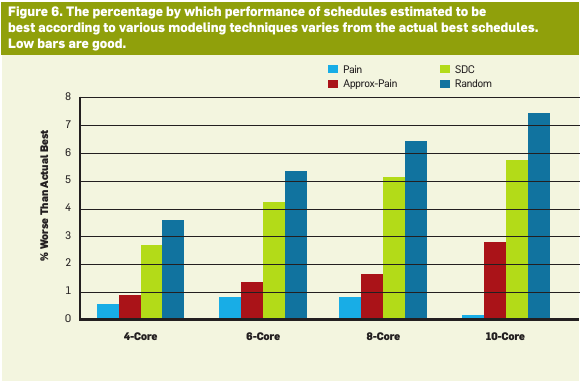
\includegraphics[height=0.7\textheight, keepaspectratio]{./pain_approx_comp}
\end{frame}


\begin{frame}
  \frametitle{scheduling based on pain metric;\\ offline vs. online measurement
    \footfullcite{zhuravlev_addressing_2010}}
  \centering
  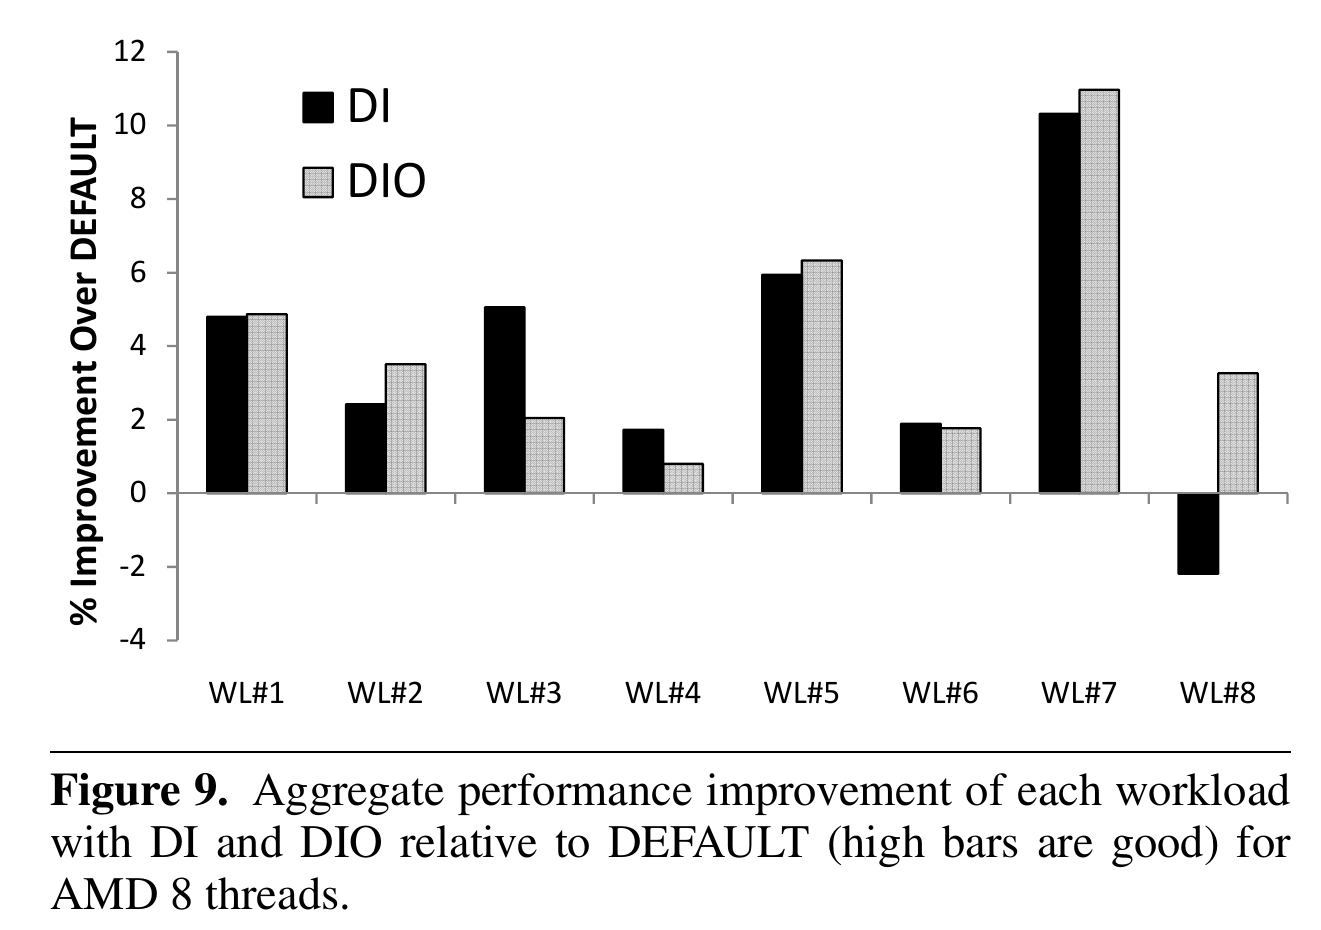
\includegraphics[height=0.7\textheight, keepaspectratio]{./opteron_di_dio}
\end{frame}


% communication
\begin{frame}
  \frametitle{thread distribution considering
    communication\footfullcite{hofmeyr_load_2010}}
    \begin{itemize}
      \item  HPC Workload: Computation--communication--cycle
      \item  balance only one application in the system
      \item  notion of speed: execution time on a core
    \end{itemize}
\end{frame}


% service architecture
%%%%%%%%%%%%%%%%%%%%%%%%%%%%%%%%%%%%%%%%%%%%%%%%%%%%%%%%%%%%%%%%%%%%%%%%%%%%%%
\begin{frame}
  \frametitle{haswell cache architecture}
  \centering
  \begin{minipage}[l]{.49\columnwidth}
    \includestandalone[width=\columnwidth]{../haswell_core_layout}
  \end{minipage}
  \begin{minipage}[r]{.49\columnwidth}
    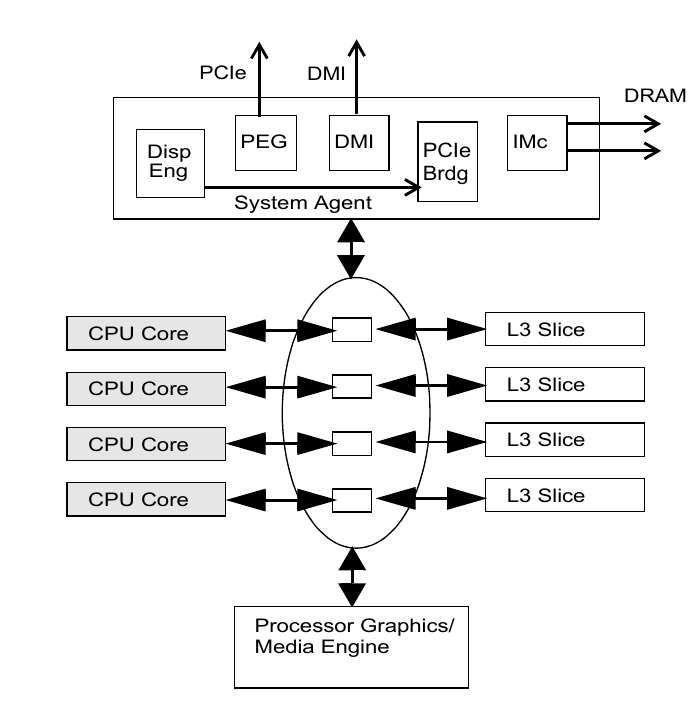
\includegraphics[scale=.27]{../haswell_architecture_by_intel_large_cropped}
  \end{minipage}
\end{frame}

\begin{frame}
  \frametitle{adjustment cycle executed each interval}
  \centering
  \includestandalone[width=.6\columnwidth]{./arch_interval_cycle}
\end{frame}


\begin{frame}
  \frametitle{threads are assigned to the core \\ with the lowest metric value}
  \centering
  \includestandalone[width=.6\columnwidth]{./placementGenerator_inside}
\end{frame}


\begin{frame}
  \frametitle{system layout}
  \centering
  \includestandalone[width=.7\columnwidth]{./threadMapper_layout}
\end{frame}


\begin{frame}[fragile]
  \frametitle{isolation \\of real-time and security critical threads}
  \centering
  \begin{minipage}[c]{\columnwidth}
    \begin{minted}[]{lua}
ld:start({  caps = { },
    scheduler = threadMapperFactory:create(
      L4.Proto.Scheduler,
      "min_prio = 0", "max_prio = 10",
      "rt = false", "sec = true" ),
    log = { "client", "green" }
  },
  "rom/ex_minimal_test");
    \end{minted}
  \end{minipage}
\end{frame}


\begin{frame}
  \centering
  What else can we do with a thread balancer?
\end{frame}

\begin{frame}
  \frametitle{PAM: performance aware meta-scheduler\footfullcite{banikazemi_pam_2008}}
  \centering
  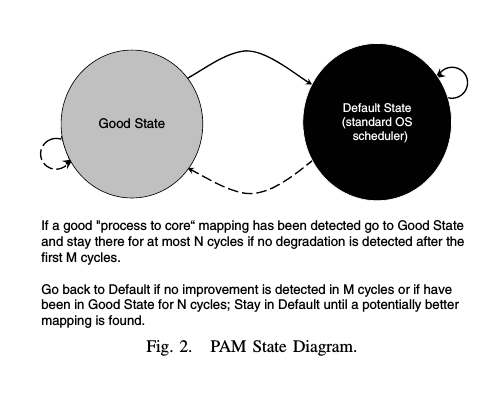
\includegraphics[scale=.5]{./pam_state}
\end{frame}

\end{document}
